\documentclass{article}

\usepackage{graphicx}
\usepackage{tikz}
\usepackage{tikzsymbols}
\usetikzlibrary{calc,patterns,shapes.geometric}
\pagestyle{empty}
\usepackage[margin=0pt]{geometry}
\geometry{papersize={14in,12in}}

\def\centerarc[#1](#2)(#3:#4:#5){\draw[#1] ($(#2)+({#5*cos(#3)},{#5*sin(#3)})$) arc (#3:#4:#5);}

\begin{document}
	\begin{figure}
		\centering
		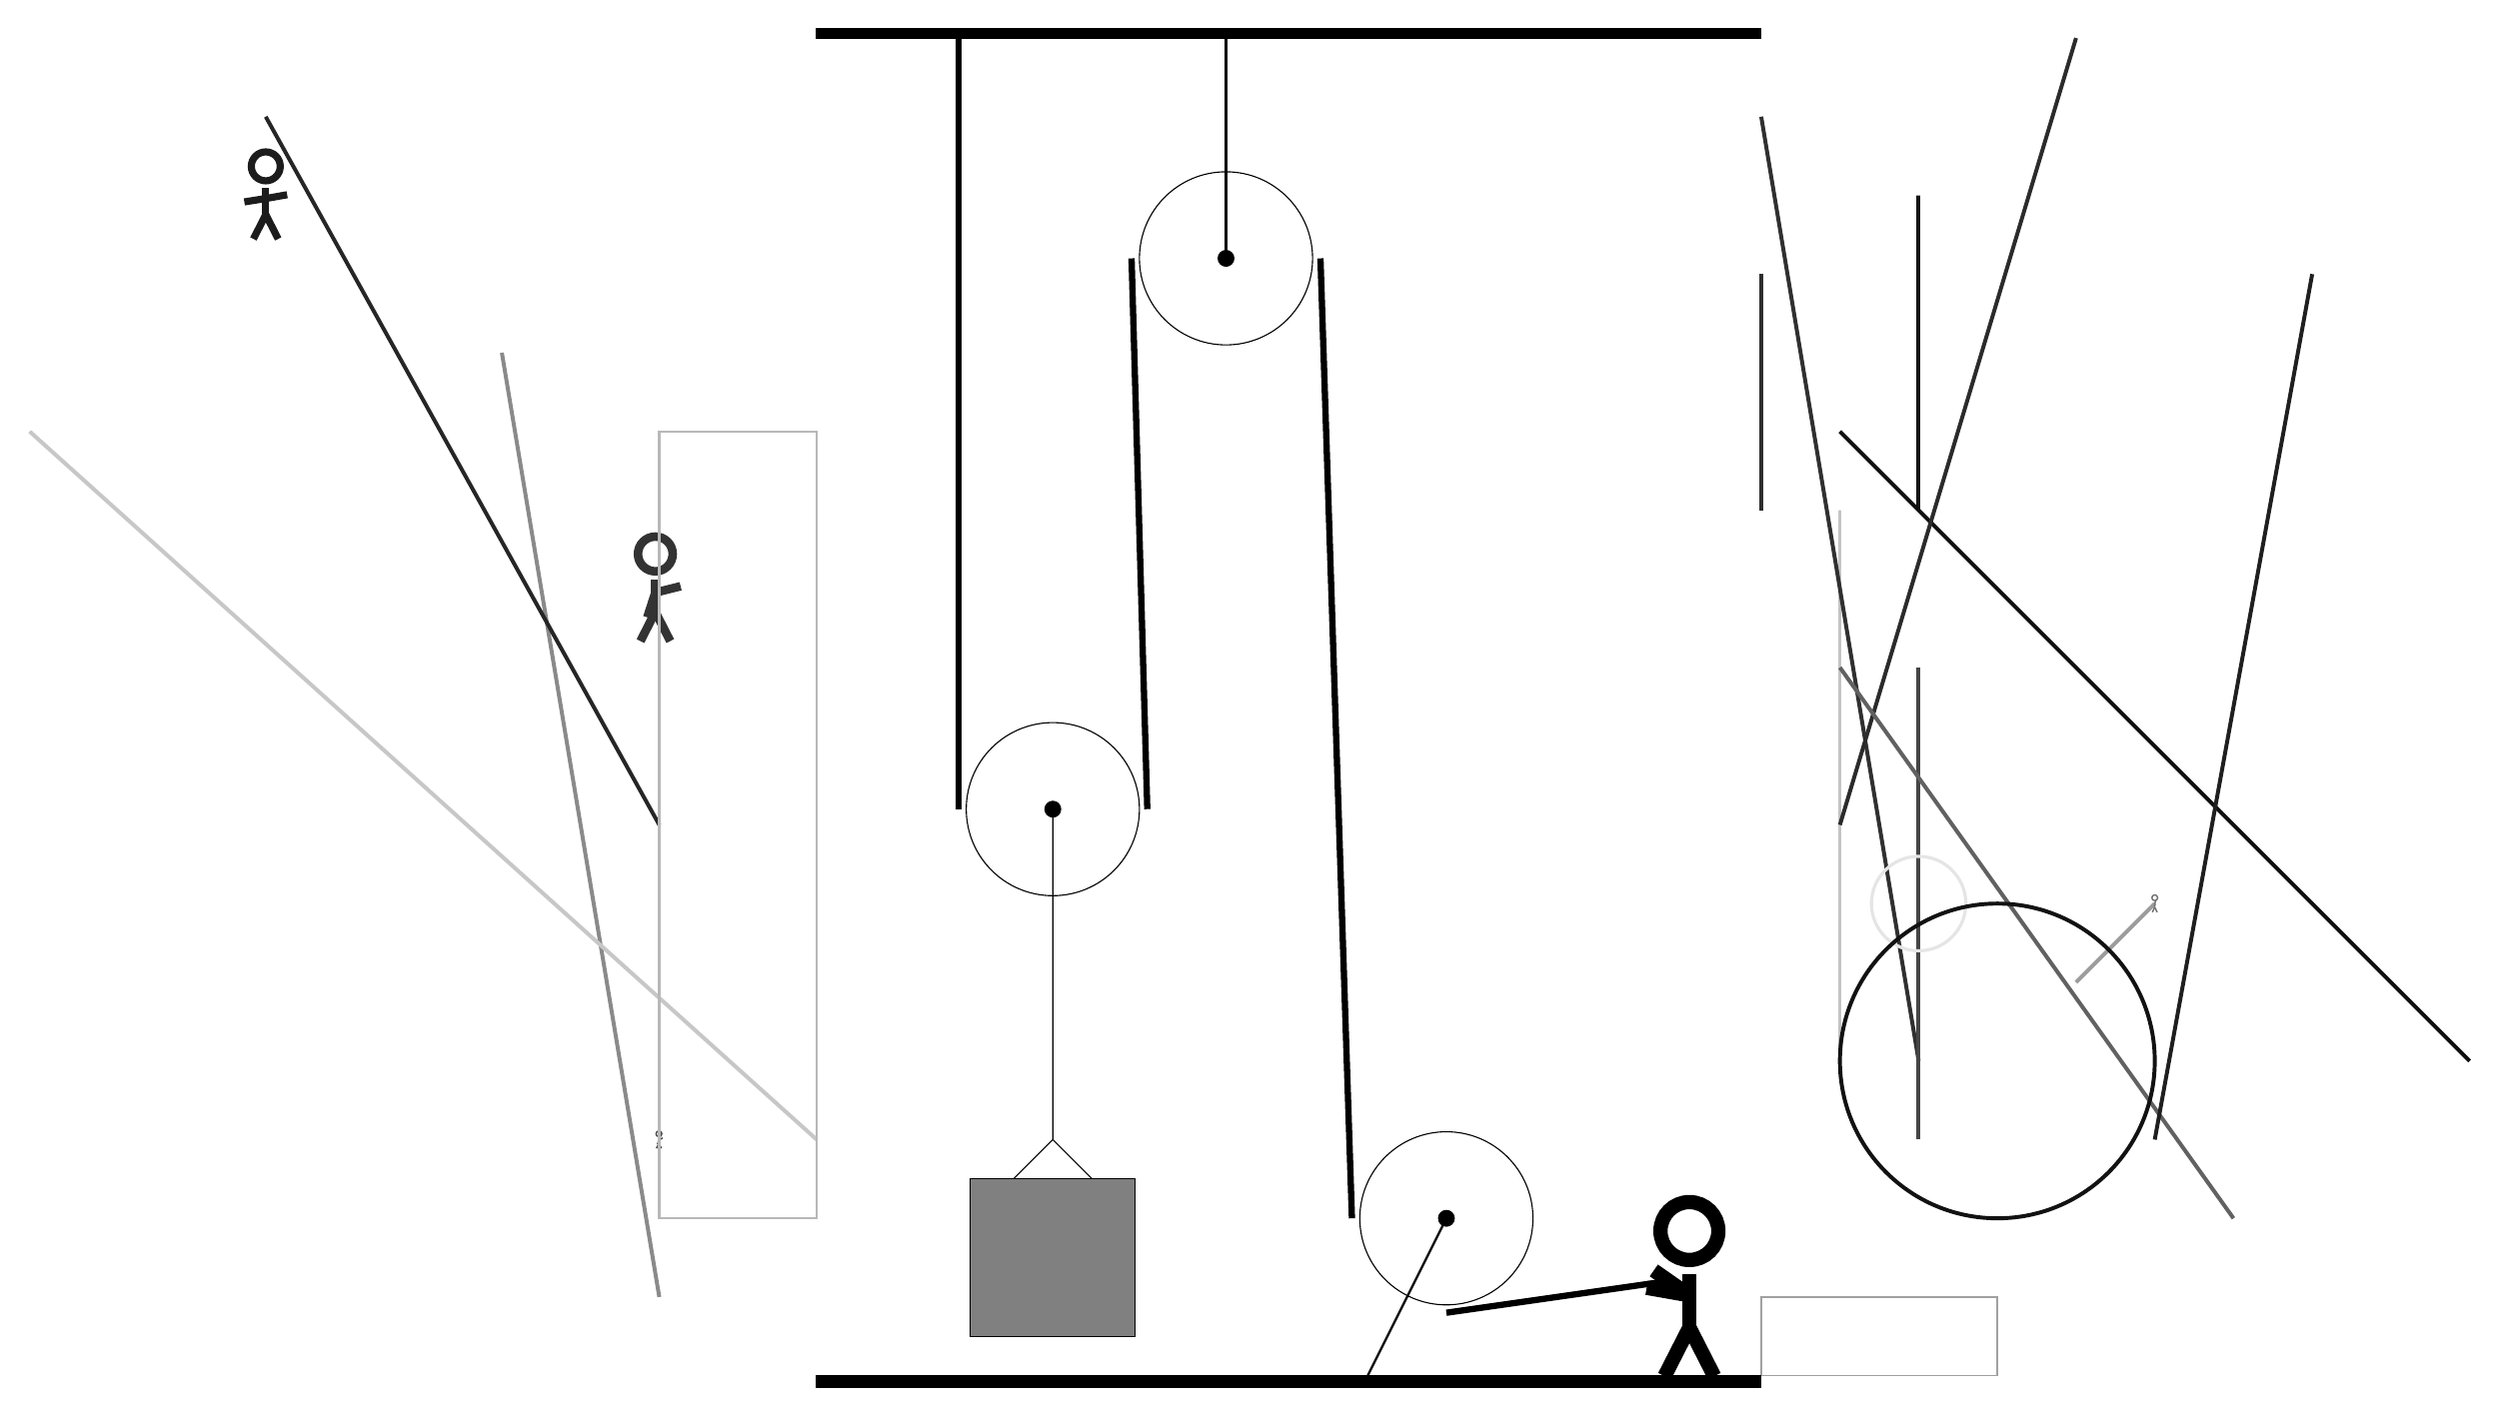
\begin{tikzpicture}
			%%%%% START %%%%%
			
			\draw[fill=black] (-2, 14) rectangle (10, 14.125);
			
			\draw (3.2, 11.2) circle (1.1);
			\draw[fill=black] (3.2, 11.2) circle (0.1);
			\draw[thick] (3.2, 11.2) -- (3.2, 14);
			
			\draw (6, -1) circle (1.1);
			\draw[fill=black] (6, -1) circle (0.1);
			\draw[thick] (6, -1) -- (5, -3);
			
			\draw (1, 4.2) circle (1.1);
			\draw[fill=black] (1, 4.2) circle (0.1);
			
			\draw (1, 4.2) -- (1, 0) -- (0.5, -0.5);
			\draw (1, 0) -- (1.5, -0.5);
			\draw[fill=black!50] (-0.05, -0.5) rectangle (2.05, -2.5);
			
			\draw[line width=0.8mm] (-0.2, 14) -- (-0.2, 4.2);
			\centerarc[line width=0.8mm](1, 4.2)(180:360:1.2000000000000002);
			\draw[line width=0.8mm](2.2, 4.2) -- (2.0, 11.2);
			\centerarc[line width=0.8mm](3.2, 11.2)(0:180:1.2000000000000002);
			\draw[line width=0.8mm](4.4, 11.2) -- (4.8, -1);
			\centerarc[line width=0.8mm](6, -1)(180:270:1.2000000000000002);
			\draw[line width=0.8mm](6, -2.2) -- (8.8, -1.8);
			
			\node at (9, -1.9) {\Strichmaxerl[10][-35][170]};
			
			\draw[line width=0.5mm, color=black!39](15, 3) -- (14, 2);
			
			\draw[line width=0.5mm, color=black!46](-6, 10) -- (-4, -2);
			\draw[line width=0.4mm, color=black!23] (11, 8) rectangle (11, 1);
			\draw[line width=0.2mm, color=black!37] (10, -2) rectangle (13, -3);
			\draw[line width=0.5mm, color=black!81](12, 1) -- (10, 13);
			\draw[line width=0.5mm, color=black!22](-2, 0) -- (-12, 9);
			\draw[line width=0.5mm, color=black!92] (12, 8) rectangle (12, 12);
			
			\node[line width=0.6mm, color=black!55] at (15, 3) {\Strichmaxerl[1][85][75]};
			\draw[line width=0.5mm, color=black!73](12, 6) -- (12, 0);
			
			\draw[line width=0.5mm, color=black!94](11, 9) -- (19, 1);
			\draw[line width=0.5mm, color=black!83](11, 4) -- (14, 14);
			\draw[line width=0.5mm, color=black!62](11, 6) -- (16, -1);
			\draw[line width=0.5mm, color=black!82](10, 11) -- (10, 8);
			
			\draw[line width=0.5mm, color=black!88](15, 0) -- (17, 11);
			\draw[line width=0.5mm, color=black!85](-4, 4) -- (-9, 13);
			\node[line width=0.7mm, color=black!80] at (-4, 7) {\Strichmaxerl[6][72][14]};
			\draw [line width=0.4mm, color=black!10](12, 3) circle (0.6);
			\draw [line width=0.5mm, color=black!93](13, 1) circle (2.0);
			\node[line width=0.5mm, color=black!71] at (-4, 0) {\Strichmaxerl[1][70][33]};
			\draw[line width=0.3mm, color=black!28] (-4, 9) rectangle (-2, -1);
			\node[line width=0.2mm, color=black!89] at (-9, 12) {\Strichmaxerl[5][9][10]};
			
			
			\draw[fill=black] (-2, -3) rectangle (10, -3.15);
			
			%%%%% END %%%%%
		\end{tikzpicture}
	\end{figure}	
\end{document}